%%% Template originaly created by Karol Kozioł (mail@karol-koziol.net) and modified for ShareLaTeX use

\documentclass[a4paper,11pt]{article}

\usepackage[T1]{fontenc}
\usepackage[utf8]{inputenc}
\usepackage{graphicx}
\usepackage{xcolor}
\usepackage{amsmath,amssymb,amsthm}
\usepackage{enumerate}
\usepackage{multicol}
\usepackage{tikz}
\usepackage[force,almostfull]{textcomp}
\usepackage{geometry}
\usepackage{hyperref}
\usepackage{soul}

\graphicspath{ {./images/} }

\geometry{total={210mm,297mm},
left=25mm,right=25mm,%
bindingoffset=0mm, top=20mm,bottom=20mm}

\renewcommand*\sfdefault{phv}
\renewcommand\familydefault{\sfdefault}

\newcommand*{\TitleFont}{%
      \usefont{\encodingdefault}{\rmdefault}{b}{n}%
      \fontsize{16}{20}%
      \selectfont}


\linespread{1.3}

\newcommand{\linia}{\rule{\linewidth}{0.5pt}}

% custom theorems if needed
\newtheoremstyle{mytheor}
    {1ex}{1ex}{\normalfont}{0pt}{\scshape}{.}{1ex}
    {{\thmname{#1 }}{\thmnumber{#2}}{\thmnote{ (#3)}}}

\theoremstyle{mytheor}
\newtheorem{defi}{Definition}

% my own titles
\makeatletter
\renewcommand{\maketitle}{
\begin{center}
\vspace{2ex}
{\huge \textsc{\@title}}
\vspace{1ex}
\\
\linia\\
\@author \hfill \@date
\vspace{4ex}
\end{center}
}
\makeatother
%%%

% custom footers and headers
\usepackage{fancyhdr}
\pagestyle{fancy}
\lhead{}
\chead{}
\rhead{}
\lfoot{Assignment 1 : WIKI,XML,CSS,XSLT }
\cfoot{}
\rfoot{Page \thepage}
\renewcommand{\headrulewidth}{0pt}
\renewcommand{\footrulewidth}{0pt}
%

% code listing settings
\usepackage{listings}
\lstset{
    language=Bash,
    basicstyle=\ttfamily\small,
    aboveskip={1.0\baselineskip},
    belowskip={1.0\baselineskip},
    columns=fixed,
    extendedchars=true,
    breaklines=true,
    tabsize=4,
    prebreak=\raisebox{0ex}[0ex][0ex]{\ensuremath{\hookleftarrow}},
    frame=lines,
    showtabs=false,
    showspaces=false,
    showstringspaces=false,
    keywordstyle=\color[rgb]{0.627,0.126,0.941},
    commentstyle=\color[rgb]{0.133,0.545,0.133},
    stringstyle=\color[rgb]{01,0,0},
    numbers=left,
    numberstyle=\small,
    stepnumber=1,
    numbersep=10pt,
    captionpos=t,
    escapeinside={\%*}{*)}
}

%%%----------%%%----------%%%----------%%%----------%%%

\begin{document}

\title{\TitleFont Assignment 1 : WIKI,XML,CSS,XSLT }

\author{Emil Sharifulllin, Innopolis University}

\date{\today}

\maketitle

\section{WIKI}

\subsection{Installation}
As a wiki engine I chose dokuwiki. I installed it as a Docker container. You can check it at \href{http://st10.os3.su:8080}{http://st10.os3.su:8080}

\begin{lstlisting}
docker run -d -p 8080:80 --name wiki mprasil/dokuwiki
\end{lstlisting}

\subsection{Organization}
Main page of wiki contain following code:
\begin{lstlisting}
======= Hello everyone ======

This wiki is about Essential Skills assignments

**List of topics which are described in this wiki:**

  * [[federated-wiki|Federated wiki]]
  * [[ward-cunningham|Ward Cunningham]]
\end{lstlisting}

\subsection{Federated wiki}
A page about federated wiki contain following wiki markup:

\begin{lstlisting}
====== Federated wiki ======

Federated wiki is a special wiki engine that allows users to fork existing pages and change forked versions. This mechanism is the same as forking mechanism in VCS. Federated wiki was designed by [[ward-cunningham|Ward Cunningham]] in 2011. 
\end{lstlisting}

\section{XML}

\addtocounter{subsection}{3}
\subsection{Animals}

Animals XML contain following data:

\begin{lstlisting}[language=xml]
<?xml version="1.0" encoding="UTF-8" ?>
<!DOCTYPE animals>
<?xml-stylesheet type="text/xsl" href="animals.xsl"?>
<animals>
    <animal name="cow">
        <skin>brown</skin>
        <noise>moo</noise>
        <eyes>beauty</eyes>
    </animal>
    <animal name="sheep">
        <skin>white</skin>
        <noise>beee</noise>
        <eyes>little</eyes>
    </animal>
    <animal name="horse">
        <skin>brown</skin>
        <noise>igogo</noise>
        <eyes>dark and incredible</eyes>
    </animal>
    <animal name="pig">
        <skin>pink</skin>
        <noise>hry</noise>
        <eyes>little and circle</eyes>
    </animal>
    <animal name="mockingbird">
        <skin>gray</skin>
        <noise>few few few</noise>
        <eyes>smart</eyes>
    </animal>
    <animal name="eel">
        <skin>yellow</skin>
        <eyes>vicious</eyes>
    </animal>
</animals>
\end{lstlisting}
\addtocounter{subsection}{1}
\subsection{DTD}
DTD to check this document

\begin{lstlisting}
<!ELEMENT animals (animal*)>
<!ELEMENT animal (skin, noise?, eyes)>
<!ATTLIST animal name CDATA #REQUIRED>
<!ELEMENT skin (#PCDATA) >
<!ELEMENT noise (#PCDATA) >
<!ELEMENT eyes (#PCDATA) >
\end{lstlisting}

\subsection{XML schema}
\begin{lstlisting}[language=xml]
<?xml version="1.0" encoding="UTF-8" ?>
<xsl:stylesheet version="1.0" 
        xmlns:xsl="http://www.w3.org/1999/XSL/Transform" 
        xmlns="http://www.w3.org/1999/xhtml">
    <xsl:output method="xml" indent="yes"
        doctype-public="-//W3C//DTD XHTML 1.0 Strict//EN" 
        doctype-system="http://www.w3.org/TR/xhtml1/DTD/xhtml1-strict.dtd"/>
    <xsl:template match="/">
        <html xmlns="http://www.w3.org/1999/xhtml" xml:lang="en" lang="en">
            <head>
                <meta http-equiv="Content-Type" content="text/html; charset=UTF-8" />
                <title>Animals</title>
            </head>
            <body>
                <h1>
                    List of animals 
                </h1>
                <xsl:apply-templates/>
            </body>
        </html>
    </xsl:template>

    <xsl:template match="animals/*">
        <table>
            <tr><th>#</th><th>Animal</th><th>Skin</th><th>Noise</th><th>Eyes</th></tr>
            <xsl:apply-templates/>
        </table>
    </xsl:template>

    <xsl:template match="animal">
        <tr>
            <td><xsl:value-of select="@name"/></td>
            <td></td>
            <td><xsl:value-of select="use"/></td>
            <td></td>
            <td></td>
        </tr>
    </xsl:template>
</xsl:stylesheet>
\end{lstlisting}

\subsection{Online validator}
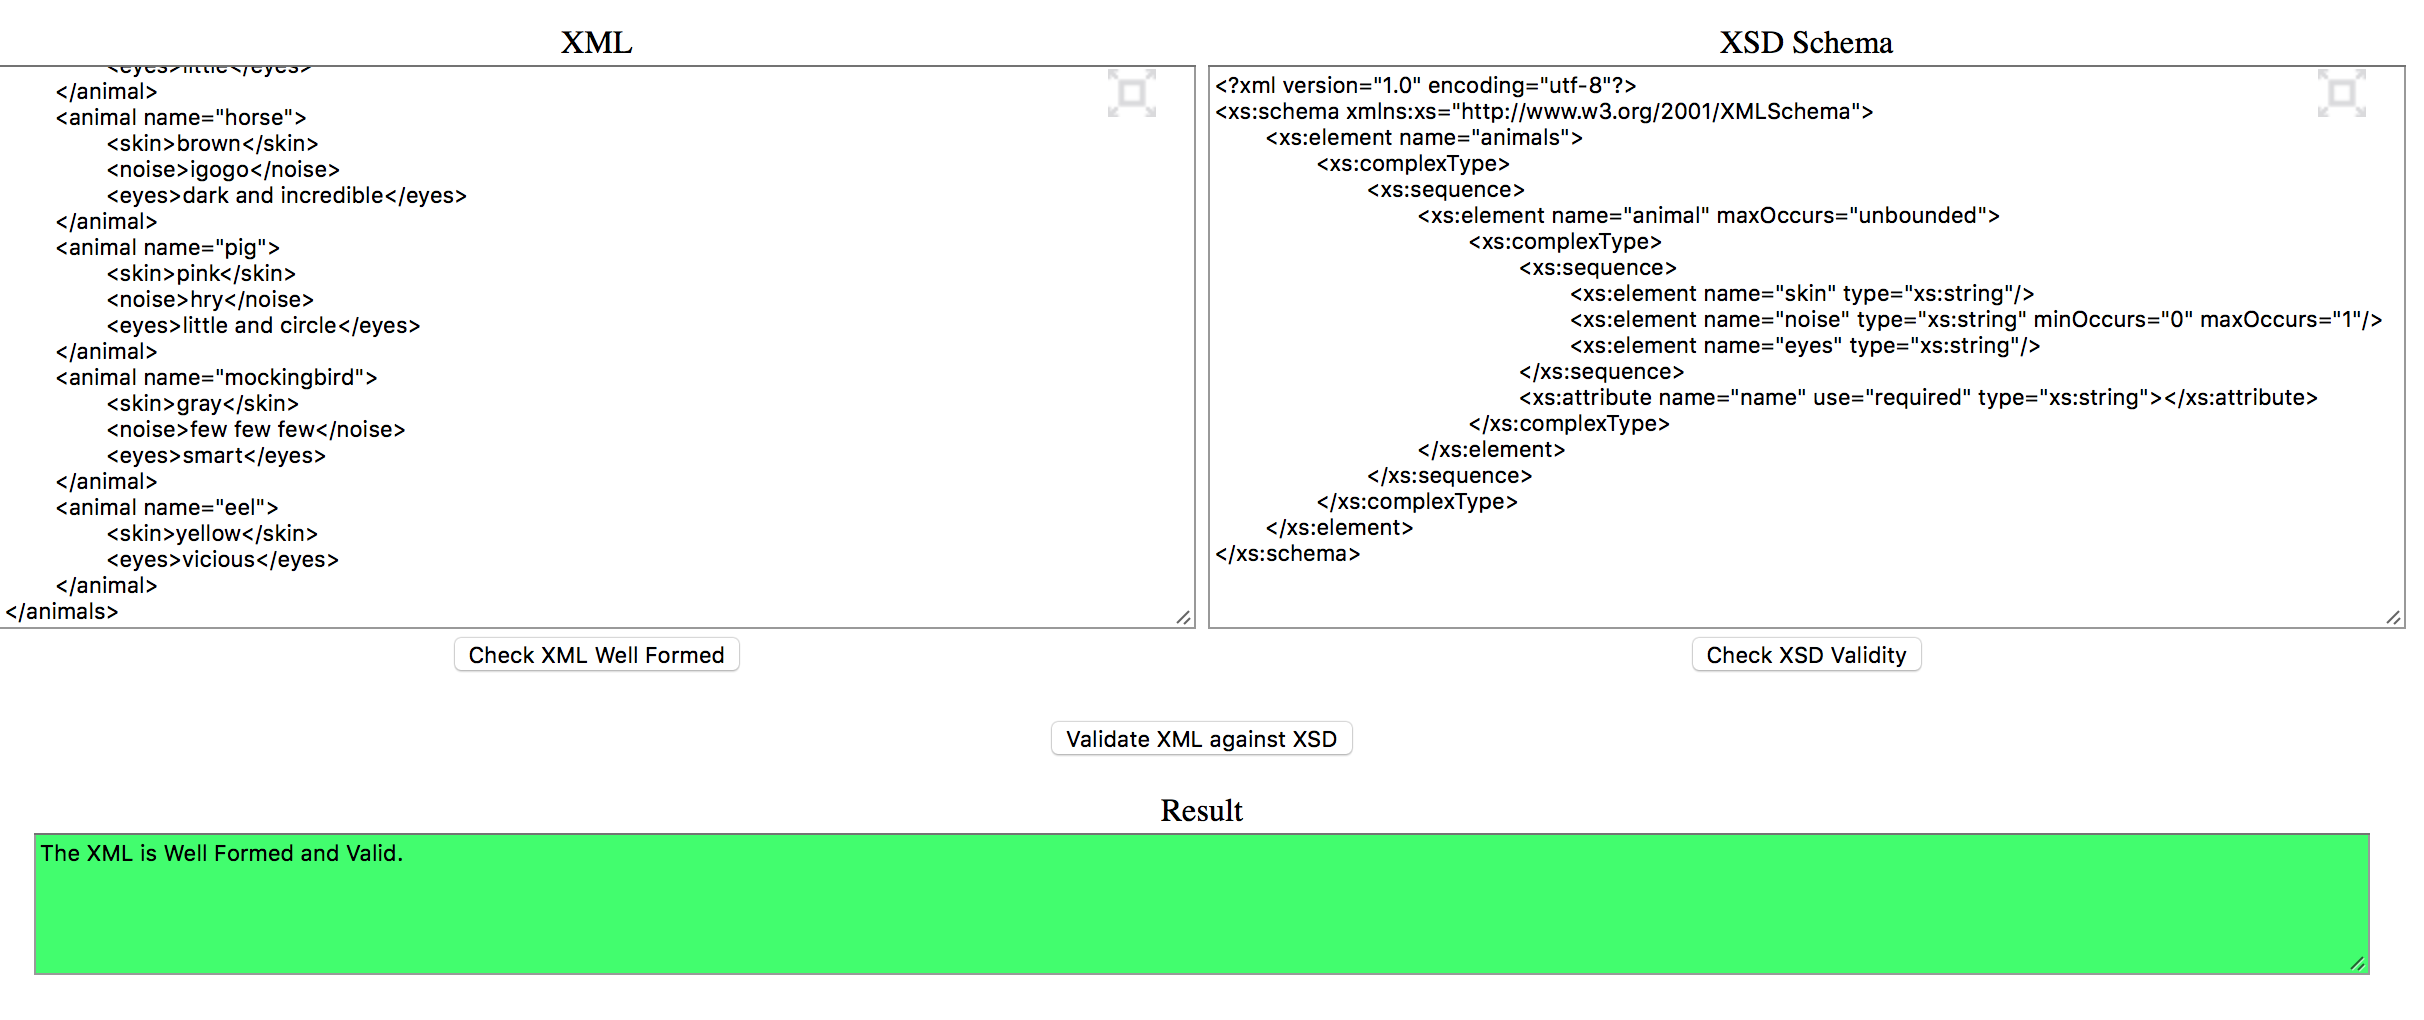
\includegraphics[width=18cm]{validator.png}
\subsection{Validating both schemas}
To validate xml with DTD I used xmllint:
\begin{lstlisting}
xmllint --dtdvalid animals.dtd animals.xml
\end{lstlisting}



\section{XSLT, CSS}
\addtocounter{subsection}{9}

\subsection{XSLT}
\begin{lstlisting}[language=xml]
<?xml version="1.0" encoding="UTF-8" ?>
<xsl:stylesheet version="1.0" 
        xmlns:xsl="http://www.w3.org/1999/XSL/Transform" 
        xmlns="http://www.w3.org/1999/xhtml">
    <xsl:output method="xml" indent="yes"
        doctype-public="-//W3C//DTD XHTML 1.0 Strict//EN" 
        doctype-system="http://www.w3.org/TR/xhtml1/DTD/xhtml1-strict.dtd"/>
    <xsl:template match="/">
        <html xmlns="http://www.w3.org/1999/xhtml" xml:lang="en" lang="en">
            <head>
                <meta http-equiv="Content-Type" content="text/html; charset=UTF-8" />
                <title>Animals</title>
                <link rel="stylesheet" href="./animals.css"/>
            </head>
            <body>
                <h1>
                    List of animals 
                </h1>
                <xsl:apply-templates/>
            </body>
        </html>
    </xsl:template>

    <xsl:template match="animals">
        <table>
            <tr><th>#</th><th>Animal</th><th>Skin</th><th>Noise</th><th>Eyes</th></tr>
            <xsl:apply-templates/>
        </table>
    </xsl:template>

    <xsl:template match="animal">
        <tr class="row">
            <td><xsl:number/></td>
            <td><xsl:value-of select="@name"/></td>
            <td><xsl:value-of select="skin"/></td>
            <td><xsl:value-of select="noise"/></td>
            <td><xsl:value-of select="eyes"/></td>
        </tr>
    </xsl:template>
</xsl:stylesheet>
\end{lstlisting}
\subsection{CSS}
\begin{lstlisting}
body {
    background-color: #84bcda;
    color: #067bc2;
}

table {
    color: #fcfff7;
    background-color: #21a0a0;
    border: solid 1px #046865;
}

td, th {border: solid 1px #046865;}

.row:hover {
    background-color: #046865;
}
\end{lstlisting}

\hl{All created documents you can see at} \href{http://st10.os3.su:8000}{http://st10.os3.su:8000}

\end{document}
